\documentclass{article}

\usepackage[dblblindworkshop,final]{neurips_2026}
\workshoptitle{AI for Science}

\usepackage[utf8]{inputenc}
\usepackage[T1]{fontenc}
\usepackage{hyperref}
\hypersetup{hidelinks}
\usepackage{url}
\usepackage{graphicx,booktabs}
\usepackage{amsmath}
\usepackage{microtype}
\usepackage{xcolor}
\usepackage{enumitem}

\makeatletter
\renewcommand{\@noticestring}{Accepted at the AI for Science workshop (NeurIPS 2026).}
\makeatother

\title{Verify Before You Build: Executable Dependency Gates for Agent-Generated Science}

\author{Mariia Baidachna \And Alina Nesen}

\begin{document}

\maketitle

\begin{abstract}
Autonomous research could accelerate scientific discovery and help solve difficult problems where the bottleneck is a researcher's time. However, the success of multi-agent systems (MAS) using interdependent methods relies on the validity of the foundational work. An erroneous claim can change which research direction seems worth pursuing, which experiment runs next, and how close a system appears to its objective. One practice in human scientific communities is to reproduce a result before building on it. We propose a similar verification strategy for research agents and implement it in Efferents, our automated research system. Its executor requires a reproduction receipt for every declared external foundation before starting downstream work. It returned the expected decision in all 13 predefined policy cases. We also tested a prompt instruction and a deterministic execution check with a language-model agent on a Minecraft crafting workflow. In the matched pilot, the no-gate and prompt-only agents each delivered 2 of 12 requested items. The enforced agent delivered none, and its executor admitted no unverified production starts. In separate assisted follow-ups, prompt-only and enforced agents each delivered all 12 items using different interfaces. We report local model token usage, test resources and wall-clock time. Verification can prevent untested production starts, but repeated tests can also consume resources without advancing the task. We aim to extend this work to mathematics and computational science.
\end{abstract}

\section{Introduction}

Consider two agents working on the same research problem. The first reports that a classifier attains a given F1 score. The second uses that number to select a baseline or decide which model to train next. If the reported score came from the wrong experiment, the error has changed the second agent's research direction before it runs a single line of code. A multi-agent system can generate ideas, code, papers and reviews in rapid succession \citep{lu2024aiscientist}. That speed makes it important to decide what evidence should travel from one agent to the next.

Human researchers have developed ways to inspect and reproduce work they intend to extend \citep{pineau2021reproducibility}. An autonomous lab can adopt a specific part of that practice. When an agent declares another lab's result essential to its next experiment, it states which procedure, inputs and output it relies on. The consuming lab runs the procedure and records whether the promised output appears. Its executor allows downstream work only while that lab holds a passing reproduction record, which we call a \emph{receipt}. An agent can still cite or discuss a paper without triggering a reproduction.

Evidence from open research tasks motivates this rule. In \emph{Into the Unknown}, nine agents each attempted 15 scientist-defined follow-up problems. None of the 135 submissions met all evaluation conditions, and 114 failed the authors' integrity check, which compared reported work and results with the available evidence \citep{kim2026unknown}. These findings raise a practical question for a lab deciding what to do next. Can the consuming lab obtain the particular result on which its proposed experiment depends? Reproduction addresses that question even when the scientific interpretation remains unsettled.

We examine this decision at two levels. In the Efferents research framework, we check whether the executor follows its policy and whether the journal responds to a changed numerical claim. In a separate Minecraft adapter, a language-model agent chooses whether to test, repair, or use a crafting method. The server records both what the method produced during reproduction and what the agent ultimately delivered. Comparing a prompt with an enforced check lets us observe when the agent proceeds without evidence, when the executor stops it, and what the agent does next.

\begin{figure}[t]
  \centering
  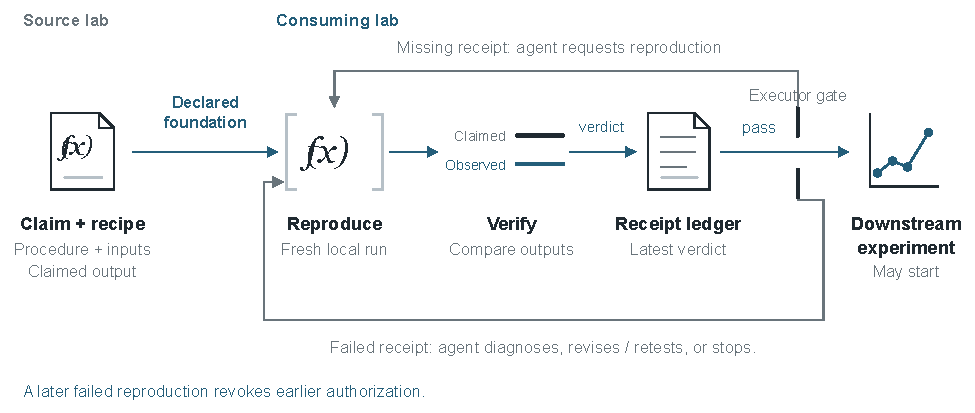
\includegraphics[width=\linewidth]{figure1.pdf}
  \caption{Reproduction executes the recipe; verification compares the output with the claim and records a verdict. The executor independently requires a current verified receipt for every declared foundation. Missing or failed evidence blocks downstream use; the agent chooses whether to test, diagnose, revise, retest or stop. All attempts remain recorded, and later failure revokes prior authorization. Reproduction does not establish scientific truth. Exact procedure-revision binding is specific to the Minecraft adapter.}
  \label{fig:flow}
\end{figure}

\section{Related work}

The NeurIPS reproducibility program combined code submission, a checklist and a community challenge \citep{pineau2021reproducibility}. FAIR sets out principles for making research objects findable and reusable, while PROV-O describes how to represent their provenance \citep{wilkinson2016fair,lebo2013provo}. ReproZip packages code and dependencies, and Whole Tale brings data, code and the execution environment into one research object \citep{rampin2016reprozip,brinckman2019wholetale}. ACM artifact review distinguishes artifact availability from independent reproduction \citep{acm2020badging}. Together these practices make work easier to rerun.

An independent effort to reimplement 255 machine learning papers found that availability of author code alone did not determine success \citep{raff2019independent}. A survey of 400 AI papers documented gaps in descriptions of methods, data and experiments \citep{gundersen2018state}. We place the decision in the consuming lab's executor. Once a proposal names another lab's result as a foundation, checking its reproduction record becomes a condition of executing the proposal.

\section{A rule for using another lab's result}

\paragraph{Publication and use.}
An author lab submits a paper with a falsifiable hypothesis and its content hash, a repository and commit identifier, claimed metrics linked to run identifiers and seeds, a description of the methods, and an executable recipe with expected outputs and tolerances. The journal checks the required fields. Critical, neutral and supportive reviewers assess the submission, and a deterministic rule combines their recommendations into a publication decision. Acceptance makes the result available for others to read.

A consuming agent names each external paper whose result is a premise of its proposal (Figure~\ref{fig:flow}). For example, an agent proposing to improve on a classifier might depend on the reported baseline F1 from that classifier's training and scoring recipe. The executor checks each declared premise against its lab's local append-only reproduction ledger. Let $D(p)$ be the declared external foundations of proposal $p$, and let $s(d)$ be the latest local status for foundation $d$. The ordinary proposal can start when

\begin{equation}
  \mathrm{allow}(p) \iff \forall d \in D(p),\ s(d)=\mathrm{verified}.
\end{equation}

An empty set satisfies the rule. A reproduction proposal may test its own target before that target has a passing receipt. Its other declared foundations still require verification. The latest result controls use. A failed reproduction after a previously successful attempt blocks the next ordinary proposal, and a later successful attempt restores permission.

\paragraph{From a rerun to a receipt.}
The journal runs the submitted recipe in a fresh directory and reads the emitted metrics. For claimed value $c$, observed value $o$, and relative tolerance $\tau$, a metric matches when
\begin{equation}
 |o-c| \leq \tau \max(|c|,10^{-9}).
\end{equation}
All required metrics must match for the journal to record a corroboration. A missing or out-of-range metric yields a challenge. A failed command prevents corroboration. Separately, the consuming executor records whether a reproduction proposal's declared metric passed, along with its measurement and run identifier. The Python ledger identifies a foundation by source lab and campaign. Changes to a method within that campaign do not automatically acquire a new identifier.

The executor checks the ledger before loading the next experiment's configuration, creating its output directories, or invoking its code. This is where an instruction to reproduce becomes binding. The agent chooses which experiment to propose; the executor determines whether that proposal has satisfied its prerequisites.

\section{Does the journal enforce the rule?}

The archived Efferents evaluation (Python 3.12.12) addresses two different failure modes. A correctly implemented executor should reject a proposal with an unverified foundation. A verifier should challenge a claim when a fresh run gives a different result. We tested the first property with predefined allow/block decisions and the second by changing one reported F1 value while holding the recipe fixed.

\subsection{Policy and bypass cases}

Table~\ref{tab:policy} groups the 13 predefined executor cases. Each case supplies a proposal, a ledger history and an expected decision. The executor returned the expected decision in all 13. Appendix~\ref{app:policy} gives each input and outcome.

\begin{table}[t]
  \caption{Policy evaluation. Allowed means the downstream experiment may start.}
  \label{tab:policy}
  \centering
  \small
  \begin{tabular}{lccc}
    \toprule
    Case group & Cases & Correct & Expected rule \\
    \midrule
    No dependency & 1 & 1 & allow \\
    Missing, pending, failed & 3 & 3 & block \\
    Verified and status updates & 3 & 3 & latest status wins \\
    Multiple foundations & 2 & 2 & all must verify \\
    Reproduction exception & 2 & 2 & target only \\
    Malformed metadata & 2 & 2 & fail closed \\
    \midrule
    Total & 13 & 13 & 100\% \\
    \bottomrule
  \end{tabular}
\end{table}

A later failure revokes authorization; a later verification restores it. A separate integration test places sentinels at configuration loading and experiment execution. An unverified proposal reaches neither sentinel, creates no experiment configuration directory, and records the reason for the block.

\subsection{Can the same method reproduce the claimed number?}

The full evaluator reruns a deterministic logistic-regression training and scoring recipe at five decision thresholds. The first fixture claims validation F1 values of 0.7273, 0.8000, 0.8889, 0.8571, and 0.6667, with a 5\% relative tolerance. All five measurements match. The second fixture changes the third claim from 0.8889 to 0.5000. The rerun again produces 0.8889, and the journal challenges that claim. Each five-run check took about 0.27 seconds on the test machine. The standalone supplement exercises the execution and verdict paths using the same five values from a lookup fixture; the archived full evaluator executes the actual training and scoring code.

\subsection{Gate cost}

Checking whether an existing receipt permits a proposal and producing a new receipt incur different costs. Table~\ref{tab:latency} measures the first operation. On one Apple arm64 laptop, each decision parses the Markdown ledger and checks the proposal. Across 1,000 timed decisions per ledger size, the median rose from 0.021~ms at one entry to 1.256~ms at 1,000 entries. These times exclude the cost of running a reproduction.

\begin{table}[t]
  \caption{Gate latency over 1,000 decisions per ledger size. Values are milliseconds.}
  \label{tab:latency}
  \centering
  \small
  \begin{tabular}{rrr}
    \toprule
    Ledger entries & Median & 95th percentile \\
    \midrule
    1 & 0.021 & 0.026 \\
    10 & 0.031 & 0.038 \\
    100 & 0.139 & 0.153 \\
    1,000 & 1.256 & 1.333 \\
    \bottomrule
  \end{tabular}
\end{table}

\section{What happens when the agent chooses its next action?}

We used Minecraft Java 1.21.6 to give the agent a dependency it could test before investing production resources. Each external method makes an executable claim: \emph{Running this code from these starting resources produces these items.} For example, a supplied crossbow procedure lists logs, raw iron, coal and string as inputs. It also needs to make a tripwire hook before the final craft. If that step is absent, the program can run through several operations before it fails. A final chest inspection can show a missing crossbow; by then the production bot has already spent time and materials. Testing the procedure earlier can reveal which prerequisite was missing.

\paragraph{What counts as evidence.}
In a standalone adapter, a verifier bot receives a fresh kit of the declared inputs in a separate arena, executes the ordered steps, and measures the change in its inventory. The production bot works from its own finite stock. A test item cannot be moved to production or counted as a delivery. An exact receipt is keyed by a hash of the method and execution context, including the episode, game version, stock, workstations, and adapter source hashes. Editing a step changes the key. Only real items recorded in the production delivery chest count toward the order. A successful test establishes that the specified method worked on that kit. Whether the agent subsequently uses the method and completes its order is a separate outcome.

Minecraft implements the rule independently of the Python journal. Known recipes and injected faults let us check the planner and executor against server observations. Scientific discovery is outside the scope of this task.

\paragraph{Matched pilot.}
We requested one of each of 12 items using a library of eight correct procedures and four with injected faults. Three episodes used the same local four-bit Qwen3.5-9B snapshot, temperature 0.2, seed setting 701, tools and budgets. Each episode started with fresh stock, conversation and receipts. With no gate, the executor admitted any method. The prompt-only arm instructed the agent to test a method before reuse while still permitting immediate production. The enforced arm used the same prompt and denied each production method call without a passing receipt. Direct actions remained available in all arms. Appendix~\ref{app:evidence} gives the resource limits and scripted controls.

\begin{table}[tb]
\centering\small
\caption{Matched pilot (seed 701). Chest counts distinct targets out of 12. Starts are admitted production method calls, classified by receipt at admission. Blocks count denied requests.}
\label{tab:episodes}
\begin{tabular}{lrrrrrr}
\toprule
Policy & Chest & Turns & Tests & Verified starts & Unverified starts & Blocks\\
\midrule
No gate & 2 & 70 & 0 & 0 & 61 & 0\\
Prompt only & 2 & 70 & 1 & 0 & 29 & 0\\
Enforced & 0 & 56 & 11 & 0 & 0 & 45\\
\bottomrule
\end{tabular}
\end{table}

The two permissive arms each delivered a hopper minecart and a chest minecart (Table~\ref{tab:episodes}). No-gate used faulty methods directly. Prompt-only tested a faulty crossbow procedure once and still attempted crossbow and dispenser procedures in production. Neither agent repaired a procedure that yielded its target. Post-episode server reads found one unit of raw iron stranded in each production furnace. The pilot toolset could not recover it. The enforced agent exhausted its token budget without a production start. It used eleven kits to test the same hopper minecart procedure eleven times. Its first unverified hopper request was blocked. The other 44 blocks concerned a correct chest minecart procedure it had never tested. All 45 blocks enforced the evidence requirement. None was a diagnosis of faulty code. Figure~\ref{fig:minecraft-workflows} follows the missing tripwire hook from this no-gate pilot to an assisted enforced run.

\begin{figure}[t]
  \centering
  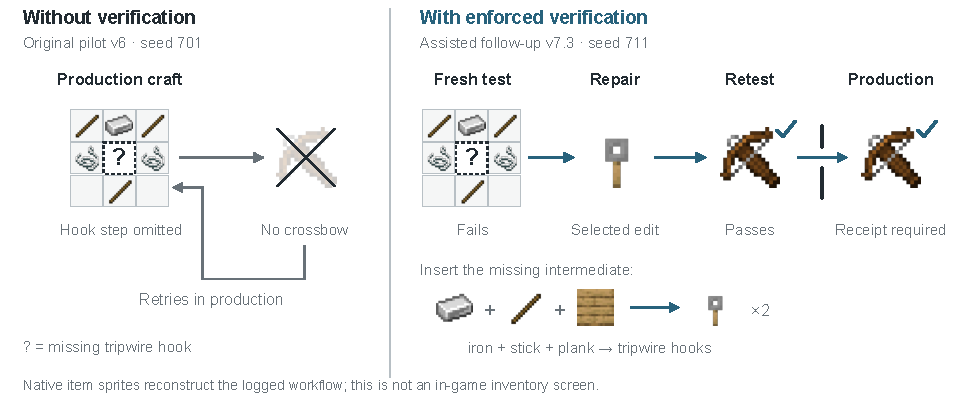
\includegraphics[width=\linewidth]{figure2.pdf}
  \caption{Item workflows reconstructed from event logs using native Minecraft 1.21.6 sprites. The supplied procedure omits the tripwire-hook craft, leaving the crossbow recipe incomplete. Without verification, the pilot retries it in production. In the assisted enforced follow-up, an isolated test catches the omission; the agent selects the hook edit, retests, and uses the exact passing receipt for production. The hook recipe yields two hooks; one is needed for a crossbow. These are annotated recipe diagrams, not captured inventory screens. Versions, seeds and interfaces differ, so the illustration does not establish a performance advantage.}
  \label{fig:minecraft-workflows}
\end{figure}

\paragraph{Development follow-up.}
At seed setting 711, a queue focused attention on the first undelivered target. After a failed test, a recipe-book helper used the failed inventory and installed vanilla recipes to suggest one missing prerequisite step. The model explicitly chose edits, tests, and production calls from a menu. The revised tools also exposed cached receipts and supported furnace recovery. These episodes measure assisted planning on the fixed order.

\begin{table}[tb]
\centering\small
\caption{All development attempts (seed 711). Chest counts targets out of 12. Daggers mark operator interruptions. Each completed run used four model-selected recipe-book edits.}
\label{tab:follow}
\setlength{\tabcolsep}{4pt}
\begin{tabular}{llrrrrrr}
\toprule
Version & Policy & Chest & Turns & Tests & Verified starts & Unverified starts & Blocks\\
\midrule
v7.1 & Prompt only$^\dagger$ & 3 & 21 & 4 & 2 & 1 & 0\\
v7.2 & Prompt only & 12 & 31 & 15 & 11 & 1 & 0\\
v7.2 & Enforced$^\dagger$ & 1 & 5 & 1 & 1 & 0 & 3\\
v7.3 & Enforced & 12 & 38 & 16 & 12 & 0 & 6\\
\bottomrule
\end{tabular}
\end{table}

We retained all four development attempts (Table~\ref{tab:follow}). The v7.1 prompt-only agent delivered three items, then repeatedly selected an unchanged dispenser edit and was stopped. Version 7.2 displayed the effect of each choice. Its prompt-only agent completed the order. The v7.2 enforced agent delivered one item and repeated a blocked chest minecart request three times before it was stopped. Its menu omitted the reason for the denial. Version 7.3 displayed that reason and the available testing action. A fresh enforced run completed the order. A second client reopened its chest and confirmed exactly one of each target.

In the completed enforced episode the model selected a recipe-book suggestion to craft the missing hook, tested the revised crossbow method, then used its passing receipt in production. Across the order, this agent made 16 fresh tests (12 passed), received six denials, and started all 12 production methods with receipts. The completed prompt-only agent made 15 fresh tests (11 passed) and started one method without a receipt. Both selected four recipe-book edits. The two completions used different feedback versions. The follow-up had no same-version no-gate baseline and used a different seed and planning tools from the pilot. We can compare their execution histories, but cannot attribute the difference in deliveries to enforcement.

\paragraph{Resources.}
A fresh test consumes a kit and planner actions. In the enforced pilot, repeating one verified method allocated 110 raw iron, 22 logs and 22 coal without advancing the production order. In the completed follow-ups, the prompt-only agent used 31 model calls in 21.7 minutes and the enforced agent used 38 calls in 23.3 minutes. Table~\ref{tab:resources} reports input and output tokens, elapsed time and primitive attempts for every episode. Inference ran locally. The records establish resource use in these episodes, not a general increase in cost or a net saving from preventing failed production.

\section{Limits and next experiments}

\paragraph{What a receipt establishes.}
A passing receipt supports the declared procedure under its tested conditions. Re-executing the same code may repeat a data leak, scoring error, or flawed experimental design. Independent implementations and external validation would test different properties. A fixed tolerance is adequate for the deterministic F1 fixture. A stochastic scientific experiment would also need prespecified seeds, a comparison rule that reflects uncertainty, and an explicit description of the conditions under which reuse is justified.

\paragraph{What the gate can miss.}
The executor sees declared foundations. An agent may omit a dependency or reproduce a different claim from the one its proposal actually needs. The Python source-lab and campaign keys also have weaker version identity than the Minecraft method-and-context hash. Verifying external artifacts on a real research network would require isolation and resource limits. The current temporary working directory alone cannot contain hostile code. The file-backed ledger is easy to audit but becomes more expensive to parse as it grows.

\paragraph{From crafting to mathematics and science.}
A mathematics agent could declare a lemma as a prerequisite to a proposed proof and provide a machine-checkable statement with its assumptions. A computational science agent could declare a baseline's code, data split, metric and tolerance before using the result in a comparison. In either setting, the next experiment should hold the planner, interface and feedback fixed across no-gate, prompt-only and enforced conditions. Independent task instances and seeds would permit estimates of both useful work completed and resources spent on verification, failed runs and recovery. These are proposed tests; the present study covers one quantitative fixture and one Minecraft order.

\section{Conclusion}

Efferents checks a reproduction receipt at the point where one agent proposes to build on another lab's result. In the Minecraft pilot the gate prevented every unverified method start, even while the planner stalled. With feedback about denials and help identifying a missing prerequisite, an agent completed the order under the same verification rule. The next question is whether checking foundations at the point of use helps research agents choose better experiments for the resources they spend.

\clearpage
\bibliographystyle{plainnat}
\bibliography{references}

\clearpage
\appendix
\section{Episode records and reproduction materials}\label{app:evidence}

\paragraph{Evidence access.}
Code and evidence are available at \url{https://github.com/Entangled-Research/verify-before-you-build}. The repository includes the framework evaluator and its archived results under \texttt{python/evaluation} and the standalone comparison fixture under \texttt{python/supplement}. The Minecraft folder includes frozen protocols and source snapshots, controls, manifests, model choices, server event streams, and terminal results. Pilot and follow-up reports index individual runs. The two completed follow-up menu audits reconcile each displayed choice with the executed action, receipt, and chest contents. Figure~\ref{fig:minecraft-workflows} uses Minecraft item textures to identify ingredients and outputs. Its production, test, and delivery events are traceable to the archived run logs. Live reproduction requires a local game installation and model weights.

\paragraph{Episodes and budgets.}
Each episode starts with a fresh conversation, stock and empty receipts. Completion requires at least one of each of 12 distinct targets in the production chest. A test receives a new input kit. A cached receipt read allocates none. Both studies allowed 70 model calls, a 200,000-token turn-start limit, 240 primitive attempts, 18 fresh test opportunities, and one hour of active time. Tests consume additional materials outside production stock. Table~\ref{tab:resources} records wall time and model usage for every Qwen episode. Interrupted attempts report observed usage and can omit an in-flight call.

\begin{table}[ht]
\centering\small
\caption{Per-episode resources. Input and output tokens are model usage, and minutes denote elapsed wall time. Primitive attempts include test and production steps.}
\label{tab:resources}
\setlength{\tabcolsep}{4pt}
\begin{tabular}{llrrrrr}
\toprule
Version & Policy & Input tokens & Output tokens & Minutes & Primitives & Cached reads\\
\midrule
v6 & No gate & 162,945 & 2,656 & 39.1 & 121 & 0\\
v6 & Prompt only & 195,735 & 6,739 & 53.9 & 102 & 0\\
v6 & Enforced & 199,793 & 1,356 & 52.7 & 66 & 0\\
v7.1 & Prompt only & 17,334 & 1,187 & 9.1 & 34 & 6\\
v7.2 & Prompt only & 21,031 & 318 & 21.7 & 125 & 0\\
v7.2 & Enforced & 3,208 & 50 & 4.0 & 12 & 0\\
v7.3 & Enforced & 26,658 & 388 & 23.3 & 130 & 0\\
\bottomrule
\end{tabular}
\end{table}

\paragraph{Controls and calibration.}
Before the matched pilot, an exact tool-selection probe fell short of its qualification criterion. A prospective amendment retained Qwen for exploratory use and documented imperfect direct-action selection. A scripted control passed all ten assertions without model calls: unverified use left production unchanged, a verified method delivered an item, a receipt failed to transfer across methods or revisions, four injected faults failed in isolation, and testing preserved production state. Calibration and scripted deliveries earn no agent credit. The first follow-up calibration passed eleven clean procedures before a missing vanilla ingredient tag caused the sand-to-glass check to fail. Version 7.1 expanded ingredient tags and passed calibration. Both calibration records are retained. Earlier setup attempts are indexed separately in the archive.

\paragraph{What the agent could repair.}
The mixed library deliberately broke the crossbow, dispenser, lectern, and blast furnace procedures. The helper searched the installed recipe book for a step that could supply the missing ingredient from the failed test inventory. It did not consult the clean procedure library. The two completed episodes each contain four explicit model selections of a suggested edit. Other targets were the hopper and chest minecarts, sticky piston, comparator, repeater, enchanting table, armor stand, and daylight detector. The archive contains input allocations, per-method outcomes, and the second client's post-terminal observation of the enforced chest.

\clearpage
\section{The thirteen predefined executor cases}\label{app:policy}
Each row is one proposal and ledger state. The framework evaluator records both the expected and observed Boolean decision. None of these cases is a Minecraft episode.
\begin{center}\small
\begin{tabular}{p{0.64\linewidth}cc}
\toprule
Proposal or latest ledger state & Expected & Observed\\
\midrule
No declared dependency & Allow & Allow\\
Foundation has no receipt & Block & Block\\
Latest status is pending & Block & Block\\
Latest status is failed & Block & Block\\
Latest status is verified & Allow & Allow\\
Verified, then failed & Block & Block\\
Failed, then verified & Allow & Allow\\
Both of two foundations verified & Allow & Allow\\
One of two foundations unverified & Block & Block\\
Reproduction tests its own target & Allow & Allow\\
Reproduction also relies on a second unverified target & Block & Block\\
Dependency container is malformed & Block & Block\\
Dependency object lacks an identifier & Block & Block\\
\bottomrule
\end{tabular}
\end{center}

\end{document}

